\chapter{Statistical Model}
\label{chap:statistical_model}

\lettrine{I}{ntroduction} into this chapter\dots

\pagebreak

\section{Time series analysis}
\label{sec:time_series_analysis}

\section{Regression and classification with Gaussian processes}
\label{sec:gaussian_processes}

\todo[inline]{introduction to GP. search over all functions. emphasize the aspects of it that we are using it for, but also a bit generally why it's good for ML. compare it to other interpolation/extrapolation methods. if makes sense, explain to what kind of data it suits.}

\subsection{Covariance functions (kernels)}
\label{subsec:covariance_functions}

Covariance functions (also called \textit{kernels}) are a key component in some mathematical concepts.
This includes \acp{gp}, where they define the statistical relationship between some input values.
In general, they represent some sort of distance or similarity $k(x, x')$ between the input points, so that $k(\cdot, \cdot)$ determines how similar the outputs $y_*$ and $y_*'$ will be. 
More formally, a covariance function can be described as $\mathcal{K}(x, x') = \phi(x) \cdot \phi(x')$, where $\phi(\cdot)$ is a function that maps the input vectors into a transformed feature space.

Which function to use is a key question when modeling using a \ac{gp}, as it determines the behavior of the model and the quality of the predictions it will be able to make.
It is important to emphasize that choosing a kernel means making some assumptions and decisions regarding the data and the way they are expected to behave.
The kernel's parameters can be optimized to achieve functions that better fit the data.
The consistency of the resulted functions can be measured with log maximum likelihood.

Some common covariance functions are given below.

\todo[inline]{current information taken from \url{http://scikit-learn.org/stable/modules/gaussian_process.html}. in the introduction add the reference(s) mention at the end of this page.}
\todo[inline]{also, there was a very detailed thesis/paper about kernels, check if there are more good details there}

\begin{description}
	
	\item[Constant Kernel -- ]
	This is a simple kernel that assigns the same value for all input pairs.
	Since by itself it does not offer a lot of characteristic to the covariance function, it is usually used as part of a product kernel, in which it scales the magnitude of the other factors, or as part of a sum kernel, in which it modifies the mean of the Gaussian process.
	It requires a single parameter, the constant value, and is defined as 
	
	\begin{equation}
	\label{eq:constant_kernel}
	k_{constant}(C, x, x') = C\forall x_1, x_2,
	\end{equation}
	\eqname{Constant kernel}
	
	where $C$ is the constant value parameter.
	A typical use case of the constant kernel is as part of a sum kernel where it explains the noise component of a signal, i.e., a \textit{white kernel}.
	In this role, the constant parameter represents the noise level and should be tuned to estimate it.
	This is determined by
	
	\begin{equation}
	\label{eq:noise_kernel}
	k_{noise}(C_{noise}, x, x') =
	\begin{cases}
	C_{noise}, & if\quad x_1 = x_2\\
	0, & otherwise.\\
	\end{cases}
	\end{equation}
	\eqname{Noise kernel}
	
	\item[Radial-basis function (RBF) kernel --]
	Also known as \textit{squared exponential kernel}, the RBF kernel is a stationary kernel.
	One derivation of this kernel has one parameter, the length scale parameter $l > 0$, which can either be a scalar (isotropic variant of the kernel) or a vector with the same number of dimensions as the inputs x (anisotropic variant of the kernel).
	It is calculated by
	
	\begin{equation}
	\label{eq:RBF_kernel}
	k_{RBF}(\{\ell, \sigma\}, x, x') = \sigma^2 exp\left(\frac{\lVert x_1 - x_2 \lVert ^2}{2\ell^2}\right),
	\end{equation}
	\eqname{Radial-basis function (squared exponential) kernel}
	
	where $\lVert x_1 - x_2 \lVert$ is the Euclidean distance between the two input points and $\sigma^2$ is a scalar factor that determines the average distance of your function away from its mean.
	\cref{fig:RBF_prior_posterior} shows prior and posterior examples of the RBF kernel.
	
	\begin{figure}[t]
		\centering
		\subfigure
		[prior of RBF kernel with $length scale = 1$]
		{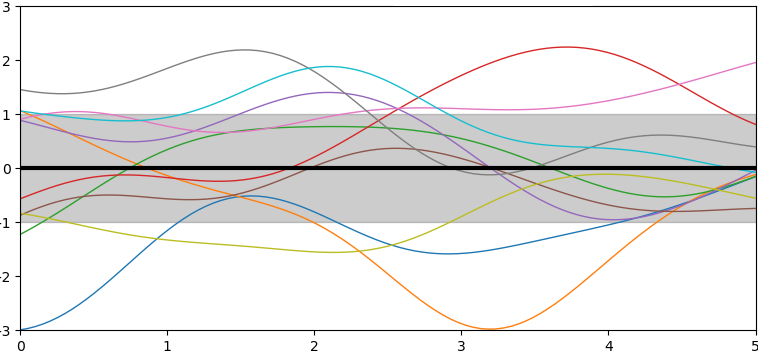
\includegraphics[width=0.45\textwidth]{RBF_prior}} 
		\hfill % no empty line here to avoid staring a new paragraph (figures will be vertically aligned)
		\subfigure
		[posterior of RBF kernel with $length scale = 0.279$]
		{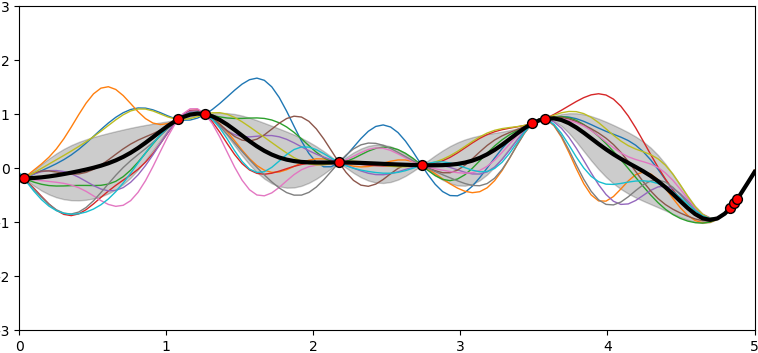
\includegraphics[width=0.45\textwidth]{RBF_posterior}}
		\caption
		[Prior and posterior of RBF kernel]
		{Prior and posterior of RBF kernel.
			This kernel typically results in smoothed functions.
			The length scale parameter determines the length of the \enquote*{wiggles} of the functions}
		\label{fig:RBF_prior_posterior}
	\end{figure}
	
	\item[Rational quadratic kernel]
	This kernel can be seen as a scale mixture (infinite sum) of RBF kernels with different length scales.
	Therefore, \acp{gp} priors with this kernel expect to see functions which vary smoothly across many length scales.
	It has two parameters: length scale $l > 0$ and scale mixture $\alpha > 0$.
	The parameter $\alpha$ determines the relative weighting of large-scale and small-scale variations.
	When $\alpha$ $\lim$ $\inf$, the RQ kernel is identical to the SE kernel, as described by
	
	\begin{equation}
	\label{eq:RQ_kernel}
	k_{RQ}(\{\sigma, \alpha, \ell\}, x, x') = \sigma^2 \left( 1 + \frac{\lVert x_1 - x_2 \lVert ^2}{2\alpha \ell^2} \right)^{-\alpha}.
	\end{equation}
	\eqname{Rational quadratic kernel}
	
	
\end{description}

Since convergence analyses usually refer to the difference between production values and not to the values themselves, only stationary kernels are used for interpolation of such measures \putref{refer to a later section where interpolation of data is performed}.
stationary kernels, also called \textit{translation invariant}, are those kernels which do not take the absolute values of the input points into account.
That is, they fulfill $k(x_1, x_2) = k(x_1 - x_2)$.
This list only covers a small subset of common covariance functions.
Further kernels include the exp-sine squared, dot-product, linear, and more.
\putref{put 2 references about kernels, or only 1 is the first is used above}

Kernels can also be chained using multiplication or addition to capture characteristics of multiple kernels.
Multiplication-based kernels are maximized when all of its kernel factors yield high values.
Addition-based kernels, however, are maximized when any of their addend kernels yield a high value.
For example, multiplying a linear kernel by a periodic one will result in functions that are \textit{both} periodic \textit{and} with increasing amplitude as they move away from the origin.

\todo[inline]{explain that we use GP to obtain ``missing'' data points in the feature vectors of the speakers to make the time series parallel and comparable.}

\section{Interpolating data using kriging}
\label{sec:interploating_data_using_kriging}

\todo[inline]{as an introduction, present Kringing, use this for a start \url{https://en.wikipedia.org/wiki/Kriging}}
\todo[inline]{definitely write down and explain the kernel we used for interpolation (probably a sum kernel of product kernel)}
\todo[inline]{don't forget to mention the log maximum likelihood of the interpolation}
